\documentclass[conference]{IEEEtran}
\makeatletter
\def\ps@headings{}
\def\@oddhead{\mbox{}\scriptsize\rightmark \hfil \thepage}%
\def\@evenhead{\scriptsize\thepage \hfil \leftmark\mbox{}}%
\def\@oddfoot{}
\def\@evenfoot{}
\makeatother
\pagestyle{headings}
\pagestyle{empty}
\usepackage{amsmath}
\usepackage{array}
\usepackage{hyperref} 
\usepackage{placeins}
\newcolumntype{P}[1]{>{\centering\arraybackslash}p{#1}}

\hyphenation{op-tical net-works semi-conduc-tor}


\usepackage{subfigure}

\usepackage{algorithmic}
\usepackage[ruled,vlined]{algorithm2e}

\ifCLASSINFOpdf
  \usepackage[pdftex]{graphicx}
  \graphicspath{ {./images/} }
  % declare the path(s) where your graphic files are
  % \graphicspath{{../pdf/}{../jpeg/}}
  % and their extensions so you won't have to specify these with
  % every instance of \includegraphics
  % \DeclareGraphicsExtensions{.pdf,.jpeg,.png}
\else
  % or other class option (dvipsone, dvipdf, if not using dvips). graphicx
  % will default to the driver specified in the system graphics.cfg if no
  % driver is specified.
  % \usepackage[dvips]{graphicx}
  % declare the path(s) where your graphic files are
  % \graphicspath{{../eps/}}
  % and their extensions so you won't have to specify these with
  % every instance of \includegraphics
  % \DeclareGraphicsExtensions{.eps}
\fi
% graphicx was written by David Carlisle and Sebastian Rahtz. It is
% required if you want graphics, photos, etc. graphicx.sty is already
% installed on most LaTeX systems. The latest version and documentation can
% be obtained at:
% http://www.ctan.org/tex-archive/macros/latex/required/graphics/
% Another good source of documentation is "Using Imported Graphics in
% LaTeX2e" by Keith Reckdahl which can be found as epslatex.ps or
% epslatex.pdf at: http://www.ctan.org/tex-archive/info/
%
% latex, and pdflatex in dvi mode, support graphics in encapsulated
% postscript (.eps) format. pdflatex in pdf mode supports graphics
% in .pdf, .jpeg, .png and .mps (metapost) formats. Users should ensure
% that all non-photo figures use a vector format (.eps, .pdf, .mps) and
% not a bitmapped formats (.jpeg, .png). IEEE frowns on bitmapped formats
% which can result in "jaggedy"/blurry rendering of lines and letters as
% well as large increases in file sizes.
%
% You can find documentation about the pdfTeX application at:
% http://www.tug.org/applications/pdftex

\begin{document}
\title{Better Approach to Geofence Detection}

% Author names 
% note positions of commas and nonbreaking spaces ( ~ ) LaTeX will not break
% a structure at a ~ so this keeps an author's name from being broken across
% two lines.
% use \thanks{} to gain access to the first footnote area
% a separate \thanks must be used for each paragraph as LaTeX2e's \thanks
% was not built to handle multiple paragraphs
\author{
Andrea Sghedoni MATR.0000736038\IEEEauthorrefmark{1},
\\
\IEEEauthorblockA{\IEEEauthorrefmark{1} DISI, University of Bologna, Italy \\
 \\
Email: andrea.sghedoni4@studio.unibo.it}}




% make the title area
\maketitle

% The Abstract
\begin{abstract}
My Location Alert is a smartphone application developed for the Android operating system.
The app allows you to create fences, selecting a center and a range, and capture all ENTER/EXIT events.\\
Whenever app detect any of these events, it is automatically sent an alert SMS to a mobile (previously selected).\\
The main goal of the project, however, is to compare the battery consumption of two strategies/services for location monitoring in time.\\
The first strategy is based on the simple polling strategy, while the second adopt a smarter auto-adaptive approach to avoid an excessive battery consumption, which would make the app unusable.

\end{abstract}



\section{Introduction}
The geofencing approach means taking monitored geographical area and giving awareness to the device of the EXIT/ENTER/REMAIN events in one area.
\textit{Location-Based Services(LBSs)} are one of the most important cause of battery discharge in smartphones.
If these services must to be continuous in time (with active jobs in background), it is probably the user's device pays a major deterioration of the battery.
In recent years, Google is committed to the improvement of these activities, especially to reach an optimum point between precision and consumption.
Please note that the location can be basically made from two mechanisms:
the first concerns the use of the GPS sensor and has an important consumption of battery in the phone, while the second concerns the use of the network(or WiFi), 
even if in this precision is less, in comparison to the use of GPS sensor.
Most of geofence mechanisms adopt a polling strategy, which controls the position at constant intervals (5 sec, 10 sec,...). 
This method, if it is merged with the use of GPS, drains battery in few hours. 
Considering also that the user, of course, does not use the smartphone only for geofencing, but developers must also take account of all the other apps that users install, use and need.\\
The main goal project is to implement an intelligent mechanism where current location is monitored frequently and with the GPS only if you are close to a fence, 
while controlling the position less frequently (and via network, to a lower consumption) as that the device moves away from the user-selected geofences.
The approach is based on an auto-adaptive mechanism, where the algorithm tries to use certain resources only when necessary, details will still in Implementation Section.
The app was developed as project part of Mobile Systems exam @ Alma mater Studiorum, Bologna.\\
The main use case of My Location Alert app is automatically alert a phone number(via SMS) of enter/exit events from a specific geographic area. 

\section{Related works}
In GooglePlay Store there are several apps that deal with the theme of geofencing, one of them is 
\textit{``EgiGeoZone Geofence``} where you can create geofences and choose between different actions(tracking, logging, email) to be made when enter/exit events are detected.
Here you need to provide the center of the fence in terms of latitude and longitude, this approach is not completely user-friendly.
Nowadays LBSs are becoming an important part of the Apps that we install every day on our smartphones, so developers need to be careful how they use 
these services and the effects they may have.
This article, see [X] in references, provided the basis for learning to better the world of localization, especially show the differences between geolocation sources, 
such as networks, WiFi and GPS.
Another interesting article is [Y], which shows proactive idea for the use of the different location technologies.\\
Can be seen as an important starting point from a developer can start to implement his own tracking strategy(or any other background service), taking account of having 
to manage different technologies at the same time.

\section{Architecture}
Basically, the app is composed with the two traditional components, such as frontend and backend.
The first component is represented by the graphic interface where users interact with maps, registration forms and so on.
The most interesting part is the back-end, \textit{Figure I}, which is composed of: \textit{Entity, SQLiteManager, Controller, Services}.

\begin{figure}
\centering
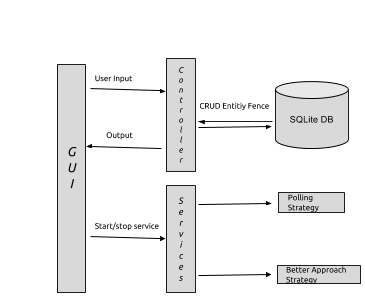
\includegraphics[scale=0.6]{architecture}
\caption{Architecture}
\end{figure}

\textit{Entity} map a fence in a java object that contains all the information needed to manage it, such as to address, latitude, longitude, range, state, activation, event to detect.\\
\textit{SQLiteManager} manages the database, provides methods for CRUD(create, read, update, delete) data of the fence.
This allows user to persist own preferences.
The DB is composed of a single table, in which each entry corresponds to a fence, registered by users and each column map an attribute of the Java class Fence.\\
The \textit{Controller} is an object that implements Singleton pattern, only one instance of that class is created and accessed.
It exposes data and methods that should be available and accessed from anywhere in the project.
Mainly, it provides the current user fence list and acts as interface to the SQLite DB, providing functions that implement CRUD verbs.\\
\textit{Services} implement the monitoring and detection strategies of registred fences, which run in the background even when the app is not open.
Only one of the two services can be active at a given time.
The performance differences between the two services implemented is the true heart of the project, you will see in the Performance evaluation section
that the polling startegy produces a battery consumption exaggerated relative to the other auto-adaptive strategy.

\section{Implementation}
Android Studio is the official IDE for Android, where you can test code on different device emulators and monitor log.
The development of a native Android App requires the use of object-oriented language JAVA.
With regard to the persistence of the user information(basically the Fence objects with their attributes) it has been necessary to create and maintain a SQLite DataBase.
We have used various services of GoogleMap Api Android, from the representation of the map(markers, fence circles) to use of location services(LocationUpdateRequests).
In addition, the Geocoding service allows the user to select the center of fence, with an address and not with latitude and longitude.
Git is used as a version control system, very important for step-by-step development and progress monitoring.\\
Location monitoring and fence events detection are the most important job that project must implement.\\
The first strategy acts polling, which get GPS position every 5 seconds(costant updates). LocationRequest, in this method, use $PRIORITY\_HIGH\_ACCURACY$ like priority parameter.\\
The second strategy is an auto-adaptive approach, which goal is a better low battery consumption.
This method uses the most expensive resources, in terms of energy(such as a GPS sensor), only when absolutely necessary. 
This means that if the device is very close to the fences will access the location more frequently, looking for accurate precision. 
Conversely if user smartphone is away from fences, the position is monitored less frequently and not with the use of GPS sensor, but taking it from the network.\\
The approach is auto-adaptive and dynamically changes the frequency and precision of the location updates.
The algorithm is based on 3 balaced parameters: \textit{distance}(between fence and current location), \textit{device speed} and \textit{direction}.
Each of these parameters are mapped on a scale from 0 to 5(see APPENDIX TABLES VI,VII,VIII), and multiplied by a coefficient, the total of the three parameters approximate sum indicates 
the frequency and the accuracy of the position updates, see TABLE I.
The coefficients provide the importance that is given to each parameter(see 1a,b,c).
The most influential parameter is the distance from the fence, but also the direction and speed parameters can become important in total evaluation, see (2).

\begin{subequations}\label{grp}
  \begin{align}
    \alpha&=0.8\label{second}\\
    \beta&=0.1\label{third}\\
    \gamma&=0.1\label{fourth}
  \end{align}
\end{subequations}

\begin{equation}
\boxed{f_i = \alpha f(distance) + \beta f(direction) + \gamma f(speed)}
\end{equation}

\begin{table}[h]
  \centering
    \begin{tabular}{|P{0.5cm}|P{1cm}|P{5.5cm}|}
    \hline
    $f_i$ & Interval (second) & LocationRequest Precision \\ \hline
    5 & 5 &  \tiny$PRIORITY\_HIGH\_ACCURACY$ \\ \hline
    4 & 30 &  \tiny$PRIORITY\_BALANCED\_POWER\_ACCURACY$ \\ \hline
    3 & 60 &  \tiny$PRIORITY\_BALANCED\_POWER\_ACCURACY$ \\ \hline
    2 & 180 &  \tiny$PRIORITY\_LOW\_POWER$ \\ \hline
    1 & 300 &  \tiny$PRIORITY\_LOW\_POWER$ \\ \hline
    0 & 480 &  \tiny$PRIORITY\_LOW\_POWER$ \\ \hline
   \end{tabular}
  \newline\newline
  \caption{Evaluation strategies}
\end{table}

\section{Performance evaluation}
\textit{MyAlertLocation} is tested on SO Android 6.0 and hardware device is LG Sprint. The removable Li-Ion battery has a nominal power of 2100 mAh, when fully charged (100\%). \\
The device has been used only for app testing, no other app has been used in test period. This way is simple get precise estimates on battery power consumption and GPS utilization. \\
Android 6, furthermore, allows to verify the consumption of these two factors for each application installed.
The tests measure the difference between the polling strategy and the auto-adaptive method, in terms of consumed battery (mAh and percentage) and use time of the GPS sensor. \\
For each test is considered a time of 20 hours and a fence placed at a determined distance, respectively 300km, 10km, 1km.\\ 
In the end,app is tested when the user moves towards,in or out fence.\\
Table II shows the differences between the two strategies, considering a fence located approximately 300 km from the location of the device.
If you use the Better Approach the energy consumption is only 0.04\%, while the poll has an exaggerated consumption, close to 30\%.
The motivation is that the service is looking for position every 5 seconds and constantly accesses to GPS, 
while the auto-adaptive method controls the position every 8 minutes, via the network with a very low battery consumption. \\
In Tables III and IV we can see that the polling strategy remains constant and produces an exaggerated consumption, 
while auto-adaptive strategy slowly increases its energy consumption according to the distance from the fence.
This is obvious: if the distance from the fence is only 1 km, it controls the position more frequently(and with more accuracy) than 10 km.
The use of GPS sensor increased because the distance to fence is only 1km and my observations should be more precise, so it might not be enough given the location via network.\\
The last test, Table V, is based on a scenario in which the user moves(entering and exiting from the fence within approximately 2km). Here, compared to the previous test (table IV), 
the consumption of battery(and GPS time) increases and this is an expected result, see Formula (2), because the user is moving in fence direction, with a certain speed so
requires the position every 5 seconds, with the maximum possible accuracy(PRIORITY\_HIGH\_ACCURACY).\\
The battery saving, compared to polling, remains optimal.

\begin{table}[h]
  \centering
    \begin{tabular}{|P{1.4cm}|P{0.8cm}|P{0.8cm}|P{0.8cm}|P{0.8cm}|P{0.8cm}|}
    \hline
    Strategy & distance (km) & Time(h) & mAh usage & \% battery & time GPS \\ \hline
    Polling & 300 & 20 & 800 & 38 & 20h   \\ \hline
    Better Approach & 300 & 20 & 1 & 0.04 & 13s   \\ \hline
   \end{tabular}
  \newline\newline
  \caption{Test 1}
\end{table}

\begin{table}[h]
  \centering
    \begin{tabular}{|P{1.4cm}|P{0.8cm}|P{0.8cm}|P{0.8cm}|P{0.8cm}|P{0.8cm}|}
    \hline
    Strategy & distance (km) & Time(h) & mAh usage & \% battery & time GPS \\ \hline
    Polling & 10 & 20 & 800 & 38 & 20h   \\ \hline
    Better Approach & 10 & 20 & 70 & 4 & 80s   \\ \hline
   \end{tabular}
  \newline\newline
  \caption{Test 2}
\end{table}

\begin{table}[h]
  \centering
    \begin{tabular}{|P{1.4cm}|P{0.8cm}|P{0.8cm}|P{0.8cm}|P{0.8cm}|P{0.8cm}|}
    \hline
    Strategy & distance (km) & Time(h) & mAh usage & \% battery & time GPS \\ \hline
    Polling & 1 & 20 & 800 & 38 & 20h   \\ \hline
    Better Approach & 1 & 20 & 160 & 8 & 5min   \\ \hline
   \end{tabular}
  \newline\newline
  \caption{Test 3}
\end{table}

\begin{table}[h]
  \centering
    \begin{tabular}{|P{1.4cm}|P{0.8cm}|P{0.8cm}|P{0.8cm}|P{0.8cm}|P{0.8cm}|}
    \hline
    Strategy & distance (km) & Time(h) & mAh usage & \% battery & time GPS \\ \hline
    Polling & IN/OUT-2km & 20 & 800 & 38 & 20h   \\ \hline
    Better Approach & IN/OUT-2km & 20 & 260 & 12 & 7min   \\ \hline
   \end{tabular}
  \newline\newline
  \caption{Test 4}
\end{table}


\section{Conclusions}
This project shows that it is desirable to use the more expensive services(in terms of the battery) in an intelligent way, otherwise the user could drain battery in a few hours.
In particular the use of the GPS sensor today is still an issue for smartphones, where some app abuse of GPS sensor. \\
The goal, in case of geofencing apps, is to use the services in an intelligent way, using GPS only when necessary and if the device is located next to a fence.
The improvements shown in the foo section is important, but there are margins of improvement.
In the future a possible feature is to check the activities that the user is doing and regular location updates based on the results obtained(it is possible with Google ActivityRecognitionApi).\\
In the end, others improvements concern a commercial point of view, with a possible integration with leading social networks, such as Twitter, Facebook, Google+.

\bibliographystyle{plain}
\begin{thebibliography}{15}

\bibitem{NomeRiferimento}
\newblock{egmontr},
\newblock{\href{https://play.google.com/store/apps/details?id=de.egi.geofence.geozone&hl=it}{\textbf{EgiGeoZone Geofence}}}
\newblock{\textit{Android App on GooglePlay}}, 2016.

\bibitem{NomeRiferimento}
\newblock{Axel Küpper, Ulrich Bareth, and Behrend Freese},
\newblock{\href{http://citeseerx.ist.psu.edu/viewdoc/download?doi=10.1.1.259.1629&rep=rep1&type=pdf}{\textbf{Geofencing and Background Tracking – The Next Features in LBSs}}}
\newblock{\textit{INFORMATIK}}, Berlin, 2011.

\bibitem{NomeRiferimento}
\newblock{Axel Küpper, Ulrich Bareth},
\newblock{\href{http://ieeexplore.ieee.org/xpl/articleDetails.jsp?tp=&arnumber=6032390}{\textbf{Geofencing and Background Tracking – The Next Features in LBSs}}}
\newblock{\textit{IEEE 35th Annual Computer Software and Applications Conference}}, Munich, 2011.

\bibitem{NomeRiferimento}
\newblock{\href{https://developer.android.com/training/location/geofencing.html}{\textbf{Creating and Monitoring Geofences}}}
\newblock{\textit{Google Android Documentation}}, 2016.

\bibitem{NomeRiferimento}
\newblock{\href{https://developer.android.com/training/location/receive-location-updates.html}{\textbf{Receiving Location Updates}}}
\newblock{\textit{Google Android Documentation}}, 2016.

\end{thebibliography}

\newpage 
\section{Appendix}
\begin{table}[h]
  \centering
    \begin{tabular}{|P{2.5cm}|P{2.5cm}|}
    \hline
    Distance(meters) & f(distance)\\ \hline
    $<$ 8000 & 5\\ \hline
    8000-30000 & 4\\ \hline
    30000-50000 & 3\\ \hline
    50000-100000 & 2\\ \hline
    100000-200000 & 1\\ \hline
    $>$ 200000 & 0\\ \hline
    \end{tabular}
  \newline\newline
  \caption{Distance evaluation}
\end{table}

\begin{table}[h]
  \centering
    \begin{tabular}{|P{2.5cm}|P{2.5cm}|}
    \hline
    Speed(Km/h) & f(speed)\\ \hline
    $>$ 130 & 5\\ \hline
    130-100 & 4\\ \hline
    100-60 & 3\\ \hline
    60-20 & 2\\ \hline
    $<$ 20 & 1\\ \hline
   \end{tabular}
  \newline\newline
  \caption{Speed evaluation}
\end{table}

\begin{table}[h]
  \centering
    \begin{tabular}{|P{2.5cm}|P{2.5cm}|}
    \hline
    Direction & f(direction)\\ \hline
    Yes & 5\\ \hline
    No & 0\\ \hline
    \end{tabular}
  \newline\newline
  \caption{Direction evaluation}
\end{table}
\end{document}
